
%*************************************************************
%
%PhD Candidate
%Computer Engineering
%Electrical & Computer Engineering Department
%Watson College of Engineering & Applied Science
%Binghamton University
%4400 Vestal Pkwy E, Binghamton, NY 13902
% Created and Developed by: Deeraj and Ronghua
%*************************************************************

%*************************************************************
% BU requirements for dissertation writing are fully adhered to!
%*************************************************************
% Import Packages and Methods
%*************************************************************
\documentclass[12pt,oneside]{book}
%*************************************************************
\usepackage{graphicx}
\usepackage{titlesec}
\titleformat{\chapter}[hang] 
{\normalfont\huge\bfseries}{\chaptertitlename\ \thechapter:}{1em}{} 

\graphicspath{ {figures/} }
\usepackage{amsmath}
\usepackage{systeme}
\usepackage{algorithm}
\usepackage{algorithmic}
%\usepackage[noend]{algpseudocode}
%*************************************************************
\makeatletter
\def\BState{\State\hskip-\ALG@thistlm}
%*************************************************************
\makeatother
\usepackage[toc,page]{appendix}
\usepackage{amssymb, amsmath, amsthm}
% these make top, right, bottom margins confirming to the requirements
\usepackage[a4paper,bindingoffset=0.0in,%
left=1.5in,right=1in,top=1in,bottom=1in,%
footskip=.25in]{geometry}

\usepackage{setspace}
\usepackage{blindtext}

% small stuff
\usepackage{amsfonts}
\usepackage{amscd}
\usepackage{mathbbol}
\usepackage{multirow}
\usepackage{hyperref}
\urlstyle{same}

\usepackage{footnote}
%************** For Appendix B Publications  *********************************************
\usepackage[sort,authoryear]{natbib}
\usepackage{bibunits}
%***********************************************************
\hypersetup{colorlinks,linkcolor={black},citecolor={black},urlcolor={black}}  

\usepackage{microtype}
% \usepackage{showkeys}  
% uncomment this when editing cross-references
\numberwithin{equation}{section}

% this makes the chapters start with a 2" margin
\makeatletter
%*************************************************************
\renewcommand*\@makechapterhead[1]{%
	\vspace*{0.75in}%
	{\parindent \z@ \raggedright \normalfont
	   \begin{center}
	    \ifnum \c@secnumdepth >\m@ne
		\huge\bfseries \thechapter.\space %\@chapapp\space \thechapter
		%\par\nobreak
		%\vskip 20\p@
		\fi
		\interlinepenalty\@M
		\Huge \bfseries #1\par\nobreak
		\vskip 40\p@
	   \end{center}
}}
\renewcommand*\@makeschapterhead[1]{%
	\vspace*{0.75in}%
	{\parindent \z@ \raggedright
		\normalfont
		\interlinepenalty\@M
		\Huge \bfseries  #1\par\nobreak
		\vskip 40\p@
}}
\makeatother
%*************************************************************
% theorem style
\theoremstyle{plain}
\newtheorem{theorem}[subsection]{Theorem}
\newtheorem{proposition}[subsection]{Proposition}
\newtheorem{lemma}[subsection]{Lemma}
\newtheorem{corollary}[subsection]{Corollary}
\newtheorem{conjecture}[subsection]{Conjecture}
\newtheorem{principle}[subsection]{Principle}
\newtheorem{claim}[subsection]{Claim}
%\newtheorem*{main-theorem-1}{Main Theorem}
%\newtheorem*{nil-to-local-repeat}{Proposition \ref{nil-to-local}}
%\newtheorem*{restate-tech-thm}{Theorem \ref{mainthm-tech}}
\theoremstyle{definition}
\newtheorem{definition}[subsection]{Definition}
\newtheorem{problem}{Problem}
\theoremstyle{remark}
\newtheorem{example}{Example}
\newtheorem{examples}{Examples}
\newtheorem*{remark}{Remark}
\newtheorem*{remarks}{Remarks}
%I prefer slanted leq and geq symbols
\renewcommand{\leq}{\leqslant}
\renewcommand{\geq}{\geqslant}

%*************************************************************
%A proof with an equation if need be.
\newsavebox{\proofbox}
\savebox{\proofbox}{\begin{picture}(7,7)%
	\put(0,0){\framebox(7,7){}}\end{picture}}
\def\boxeq{\tag*{\usebox{\proofbox}}}
%*************************************************************
%Modular arithmetic .
\newcommand{\md}[1]{\ensuremath{(\operatorname{mod}\, #1)}} % \operatorname automagically uses the right font and size
%\def\proof{\noindent\textit{Proof. }}
\def\endproof{\hfill{\usebox{\proofbox}}}
\def\E{\mathbb{E}}
\def\so{\mathfrak{so}}
\def\sp{\mathfrak{sp}}
\def\Z{\mathbb{Z}}
\def\R{\mathbb{R}}
\def\T{\mathbb{T}}
\def\C{\mathbb{C}}
\def\N{\mathbb{N}}
\def\P{\mathbb{P}}
\def\F{\mathbb{F}}
\def\Q{\mathbb{Q}}
\def\b{{\mathbf b}}
\def\A{{\mathbf A}}
\def\g{{\mathfrak g}}
\def\hp{{\mathfrak{hp}}}
\def\D{\mathcal{D}}
\def\re{\operatorname{Re}}
\def\O{\mathcal{O}}
%*************************************************************
\newcommand\DD{{\frac{\partial}{\partial z}}}
\newcommand\DDbar{{\frac{\partial}{\partial \overline{z}}}}
\newcommand\SPEC{{\textrm{Spec}}}
\newcommand\MM{{\mathscr M}}
\newcommand\OO{{\mathscr O}}
\newcommand\LL{{\mathcal L}}
\newcommand\PP{{\mathbf P}}
\newcommand\eps{{\varepsilon}}
\newcommand\supp{\mathop{\rm supp}}
\newcommand\Riem{{\operatorname{Riem}}}
\newcommand\dist{{\operatorname{dist}}}
\newcommand\Hess{{\operatorname{Hess}}}
\newcommand\Ric{{\operatorname{Ric}}}
\newcommand\Vol{{\operatorname{Vol}}}
\renewcommand\min{{\operatorname{min}}}
%\newcommand{\INDSTATE}[1][1]{\STATE\hspace{#1\algorithmicindent}}

%***********************imported from ronghua*****************
\newtheorem{defn}{\textbf{Definition}}[chapter]
\newtheorem{ruln}{\textbf{Rule}}[chapter]
\newcommand{\argmin}{\operatornamewithlimits{argmin}}
\renewcommand{\thealgorithm}{\arabic{chapter}.\arabic{algorithm}}
\newcommand{\INDSTATE}[1][1]{\STATE\hspace{#1\algorithmicindent}}
%*************************************************************
\parindent 0mm
\parskip   5mm % this should make \ni and  obsolete, hopefully
%\newenvironment{proof}{\noindent {\bf Proof} }{\endprf\par}
\def \endprf{\hfill  {\vrule height6pt width6pt depth0pt}\medskip}
% add a customized "itemize" operator. 
\def\+{+}
\makeatletter
\catcode`\ =12\let\@nl@space= \catcode`\ =10
\newcount\@nl@rlevel
\newcount\@nl@llevel
\@nl@llevel=-1

\def\@nl{%
	\catcode`\ =12
	\global\@nl@rlevel=0
	\futurelet\@nl@store\@nl@%
}
\def\@nl@gobble#1{\futurelet\@nl@store\@nl@}
\def\@nl@enditemize{
	\ifnum\the\@nl@rlevel<\the\@nl@llevel%
\end{itemize}%
\egroup%
\expandafter\@nl@enditemize%
\else%
\ifnum\the\@nl@rlevel=\the\@nl@llevel\else%
\errmessage{Error: inconsistent identation}
\fi%
\fi%
}
\def\@nl@{%
\ifx\@nl@store\@nl@space%
\global\advance\@nl@rlevel by 1
\expandafter\@nl@gobble%
\else%
\catcode`\ =10
\ifx\@nl@store+%
\ifnum\the\@nl@rlevel>\the\@nl@llevel%
\bgroup%
\@nl@llevel=\the\@nl@rlevel
\begin{itemize}%
	\fi%
	\@nl@enditemize%
	\item \expandafter\expandafter\expandafter\@gobble%
	\else%
	\ifx\@nl@store\@nl%
	\global\@nl@rlevel=-1\relax\@nl@enditemize\par
	\else\space\fi%
	\fi%
	\fi%
}
\makeatother
%*************************************************************


%*************************************************************
% Set Chapter Counter.
%*************************************************************
\setcounter{chapter}{0}
% makes page numbers appear
\pagestyle{plain} 
%*************************************************************

\begin{document}
% makes the page numbers roman numerals, doesn't count
% these pages in the table of contents
\frontmatter
\thispagestyle{empty}
\vbox to 1truein{}

%*************************************************************
% Beginning of Dissertation Cover/Title Page
%*************************************************************
%*************************************************************
% Dissertation Title
%*************************************************************
%\begin{doublespace}
\centerline{Disseration Title} 
%\centerline{second line if its long}

%\end{doublespace}
%*************************************************************
\vskip 200pt


\centerline{BY}
\vskip 10pt

\centerline{FirstName LastName}
\vskip 10pt
\centerline{BTech, ABC University, 2015}
\centerline{MS, XYZ University, 2017}
\vskip 10pt



\vskip 180pt

%\centerline{PROSPECTUS}
\centerline{DISSERTATION}
\vskip 10pt
%\begin{doublespace}
\centerline{Submitted in partial fulfillment of the requirements for}
\centerline{the degree of Doctor of Philosophy in Electrical and Computer Engineering}
\centerline{in the Graduate School of}
\centerline{Binghamton University}
\centerline{State University of New York}
\centerline{202X}
%\end{doublespace}
%*************************************************************
% End of Dissertation Cover/Title Page
%*************************************************************

%*************************************************************
% Beginning of Empty Page, just next Title Page
%*************************************************************
\newpage

\thispagestyle{empty}

\vbox to 9.0truein{}

\centerline{\copyright\ Copyright by Author Name 202X}

\centerline{All Rights Reserved}
%*************************************************************
% End of Empty Page, just next Title Page
%*************************************************************

%*************************************************************
% Beginning of Committee Page
%*************************************************************
\newpage

{\baselineskip = 10pt

\vbox to 2.0truein{}


\vskip 270pt

\centerline{Accepted in partial fulfillment of the requirements for}
\centerline{the degree of  Doctor of Philosophy in Electrical and Computer Engineering}
\centerline{in the Graduate School of}
\centerline{Binghamton University}
\centerline{State University of New York}
\centerline{202X}

\

\centerline{Oct 10, 202X}

\

\centerline{FirstName LastName, Ph.D., Chair}
\centerline{Department of Electrical and Computer Engineering, Binghamton University}


\

\centerline{FirstName LastName, Ph.D.,  Member}
\centerline{Department of Electrical and Computer Engineering, Binghamton University}

\

\centerline{FirstName LastName, Ph.D., Member}
\centerline{Department of Electrical and Computer Engineering, Binghamton University}

\

\centerline{FirstName LastName, Ph.D., Outside Examiner}
\centerline{Department of XYZ, ABC University}
}

%*************************************************************
% End of  Committee Page
%*************************************************************


%*************************************************************
% Abstract
%*************************************************************
\chapter*{\centering{Abstract}}
%*************************************************************
\begin{doublespace}

Add your abstract here.
	

\end{doublespace}

%*************************************************************
% Dedication
%*************************************************************
\newpage

\chapter*{\centering{Dedication}}
\bigskip
\begin{doublespace}
\centerline{\textbf{To}}
\centerline{Name here}

Few words for your dedication.

\bigbreak
\bigbreak
\centerline{Yours,}
\centerline{Author Name}
\end{doublespace}


%*************************************************************
% Acknowledgements
%*************************************************************
\newpage

\chapter*{\centering{Acknowledgements}}
\begin{doublespace}	
	
Acknowledge everyone who helped you reach this milestone. Your contributions are enabled by many people supporting your hardwork.  
	
\end{doublespace}

%*************************************************************
% Acknowledgements
%*************************************************************
\newpage


%*************************************************************
%Table of content
%*************************************************************
\tableofcontents

 
%*************************************************************
%List of Figures
%*************************************************************
 % Make the list of figures
\clearpage %\cleardoublepage %for openright
\addcontentsline{toc}{chapter}{\listfigurename} 
\listoffigures
 %\thispagestyle{plain}

%*************************************************************
%List of Tables
%*************************************************************
% Make the list of tables
\clearpage %\cleardoublepage %for openright
\addcontentsline{toc}{chapter}{\listtablename}
\listoftables
 %\thispagestyle{plain}
 \clearpage %\cleardoublepage %for openright


%*************************************************************
%All The Chapters in Order 
%*************************************************************

% Changes page numbers to regular numbers, resets the counter
\mainmatter
% This gives 11pt font with 20pt spacing, text from here should be double spaced
\fontsize{11}{20pt} \selectfont  
% \include puts in the .tex file with the given name
% make sure that these files don't have any preamble material
\begin{doublespacing}
%*************************************************************
% Author Name
%*************************************************************
%Chapter One
%*************************************************************
%*************************************************************
% Introduction
%*************************************************************
%*************************************************************
\chapter{Introduction}
\label{ch:intro}
%*************************************************************



%*************************************************************
\section{Sample Section}
\label{sec:ch1_section_one}
%*************************************************************
Add your text here. To make any citations, you need to import the bibtex of your reference to the 'Ref.bib' file. Then use the citekey \cite{nagothu2018microservice} to add your citations \cite{nagothu2021authenticating}.

You can refer to your figure usig \ref{fig:ch1_figure}. The the following commands to import the figures from 'figs' folder. Try to follow a naming convention for each figure based on their chapter appearance. If the figure is too big, then you can adjust its size by changing the 'width' parameter. 

\begin{figure}[t]
    \centering
        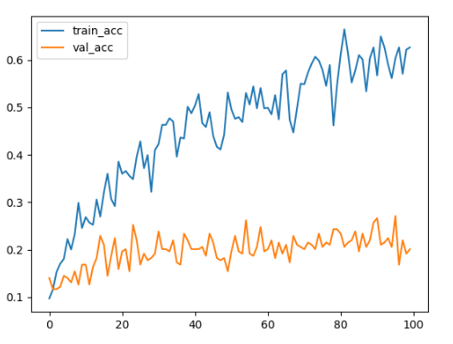
\includegraphics[width=0.98\textwidth]{figs/acc.png}
    \caption{A sample for figure.}
    \label{fig:ch1_figure}
    \vspace{-10pt}
\end{figure}


%*************************************************************
\section{Challenges and Motivation}
\label{sec:ch1_challenges}
%*************************************************************



%*************************************************************
\section{Major Contributions}
\label{sec:ch1_contributions}
%*************************************************************
 A summary of the contributions made in this dissertation is as follows,

\begin{itemize}
    \item A comprehensive study of existing techniques
    \item Item 2
    \item Item 3
    
\end{itemize}

%*************************************************************
% End of Introduction
%*************************************************************
%*************************************************************

%*************************************************************
%Author Name
%*************************************************************
%Chapter Two
%*************************************************************
%*************************************************************
% Background and Related Works
%*************************************************************
%*************************************************************
\chapter{Background and Related Works}
\label{ch:background_related}
%*************************************************************


%*************************************************************
%2.1: Existing Challenges 
%*************************************************************
\section{Current State Security}
\label{sec:ch2_current_state}
%*************************************************************




%*************************************************************
% End of Background and Related Works
%*************************************************************
%*************************************************************

%*************************************************************
%Deeraj Nagothu
%*************************************************************
%Chapter Three
%*************************************************************
%*************************************************************
% System Architectures
%*************************************************************
%*************************************************************
\chapter{Chapter three with Tables and Equations}
\label{ch:chapter_three}
%*************************************************************
%3.1: Sample section with tables and equations
%*************************************************************
\section{Section in Chapter three}
\label{sec:label_here}
%*************************************************************


% Sample table 
   
\begin{table} \small \sf

\begin{center}
\begin{tabular}{|c|c|c|c|}
\hline
\textbf{Nominal} & \textbf{Frame}& \textbf{Aliasing}& \textbf{2nd} \\
\textbf{Frequency (Hz)} & \textbf{Rate}& \textbf{Frequency (Hz)}& \textbf{Harmonic} \\
\hline
60& 29.97&0.12 &0.24  \\
\hline
60& 23.97&0.12 &0.24  \\
\hline
60& 30&0 &0  \\
\hline
60& 25&5 &10  \\
\hline
50& 29.97&10.09 &9.79  \\
\hline
50& 23.97&4.12 &8.24  \\
\hline
50& 25&0 &0  \\
\hline
50& 30&10 &10  \\
\hline
\end{tabular}
\caption{Aliased Frequency for a given Video Frame rate with different nominal frequency.}
\label{tab:ch3_table}
\end{center}
\vspace{-10 pt}
\end{table}

Sample Equation here,

$$f_{a} = | f_{l} - k \cdot f_{FPS} | < \frac{f_{FPS}}{2}$$   

\noindent where $ f_{a} $ is the aliasing frequency, $ f_{l} $ is the illumination frequency, $ f_{FPS} $ is the sampling rate of video recorders, i.e. video FPS, and $k$ varies until the condition is satisfied. Table \ref{tab:ch3_table} presents different $ f_{a} $ for their respective nominal frequency. It is evident that with a CCD-based imaging sensor, the ENF component appears at different frequencies as long as it doesn't disappear as the DC component with $30$ FPS. 


A sample for equation with Equation number 

\begin{equation}
  Y(\omega) =  \sum_{m=0}^{M-1}   X\left( \frac{\omega L - 2 \pi m}{M} \right) F_m(\omega) \label{eq:ch3_freq_filter_bank}   
\end{equation}
  
\noindent where $$F_m(\omega) =   \frac{1}{M}  \sum_{l=0}^{L-1}  e^{-j\frac{\omega(M - L) + 2 \pi m}{M}l} $$


%*************************************************************
% End of chapter 3
%*************************************************************
%*************************************************************

%*************************************************************
%Author Name
%*************************************************************
% Chapter Four
%*************************************************************
%*************************************************************
% Chapter 4
%*************************************************************
%*************************************************************
\chapter{Chapter Four}
\label{ch:chapter_four}
%*************************************************************
%*************************************************************
%4.1: Testbed Implementation 
%*************************************************************
\section{Testbed Implementation }
\label{sec:ch4_testbed}
%*************************************************************


%*************************************************************
% End of chapter 4
%*************************************************************
%*************************************************************

%*************************************************************
% Author Name
%*************************************************************
% Chapter Five
%*************************************************************
%*************************************************************
% 
%*************************************************************
%*************************************************************
\chapter{Detection}
\label{ch:detection}

%*************************************************************
%5.1: Testbed Implementation 
%*************************************************************
\section{Testbed Implementation }
\label{sec:ch5_testbed}
%*************************************************************


%*************************************************************
% End of chapter 5
%*************************************************************
%*************************************************************

%*************************************************************
% Author Name
%*************************************************************
% Chapter Six
%*************************************************************
%*************************************************************
% Consensus mechanism
%*************************************************************
%*************************************************************
\chapter{Consensus Mechanism}
\label{ch:consensus}
 Table \ref{tab:ch6_testbed} represents the devices used for the experimental study. 

\begin{table}[t]
    \caption{Configuration of Experimental Nodes.} 
    \vspace{-0.18in}
    \label{tab:ch6_testbed}
    \begin{center}       
    \begin{tabular}{|l|p{5.0cm}|p{5.0cm}|} %% this creates two columns
    \hline
    \rule[-1ex]{0pt}{3.5ex} \textbf{Device} & Dell Optiplex-7010 & Raspberry Pi 4 Model B \\
    \hline
    \rule[-1ex]{0pt}{3.5ex} \textbf{CPU} & Intel Core TM i5-3470 (4 cores), 3.2GHz & Broadcom ARM Cortex A72 (ARMv8) , 1.5GHz \\
    \hline
    \rule[-1ex]{0pt}{3.5ex} \textbf{Memory} & 8GB DDR3 & 4GB SDRAM \\
    \hline
    \rule[-1ex]{0pt}{3.5ex} \textbf{Storage} & 350G HHD & 62GB (microSD card) \\
    \hline
    \rule[-1ex]{0pt}{3.5ex} \textbf{OS} & Ubuntu 16.04 & Raspbian (Jessie) \\
    \hline
    \end{tabular}
    \end{center}
    \vspace{-0.10in}
\end{table}


%*************************************************************
% 6.5: Discussion
%*************************************************************
\section{Discussion}
\label{sec:ch6_discussion}
%*************************************************************

Add your discussions here


%*************************************************************
% End of chapter 6
%*************************************************************
%*************************************************************

%*************************************************************
%AUTHOR NAME
%*************************************************************
%Chapter Seven
%*************************************************************
%*************************************************************
% 
%*************************************************************
%*************************************************************
\chapter{Chapter 7}
\label{ch:chapter_seven}

%*************************************************************
% End of Chapter 7
%*************************************************************
%*************************************************************

%*************************************************************
%Author Name
%*************************************************************
%Chapter Eight
%*************************************************************
%*************************************************************
% Conclusions
%*************************************************************
\chapter{Conclusion and Future Work}
\label{ch:conclusion}
%*************************************************************

\section{Major Contributions}

Summarize your dissertations major contributions here. 


\section{Future Work}
If required for further discussions. 
%*************************************************************
% End of Chapter 8
%*************************************************************
%*************************************************************

\end{doublespacing}

%*************************************************************
%*************************************************************
\begin{appendices}
%*************************************************************
%*************************************************************
\begin{doublespacing}

% For Acronyms throughout the dissertation
%*************************************************************
%Author Name
%*************************************************************
%Appendix A
%*************************************************************
%*************************************************************
% Acronyms
%*************************************************************
%*************************************************************
\chapter{Appendix: Acronyms}
\label{app:a}
%*************************************************************

A\&V - Audio and Video \newline
AED - Audio Event Detectors \newline
AI - Artificial Intelligence \newline
XMP - Extensible Metadata Platform 
% For including your publications as part of disseration. The code in Appendix_B.tex makes your name bold. Please refer to that file to add your name and include the tag '\myname' in the bibtex.
\chapter{Appendix: Publications}
\label{app:b}

\newcommand{\myname}{\textbf{Deeraj Nagothu}}

\begin{bibunit}[plain]
\renewcommand{\bibsection}{\large \textbf{Journal Publications}}
\makeatletter
\renewcommand\@biblabel[1]{#1.}
% \newcommand{\BibLabel}{%
%     \hfill
%     \Hy@raisedlink{\hyper@anchorstart{cite.\CurrentBib}\hyper@anchorend}
%     [\thebib]
% }
\makeatother
\def\bibfont{\small}

%list all the references in the publications bibtex file
\nocite{*}
\putbib[journal]
\end{bibunit}

\begin{bibunit}[plain]
\renewcommand{\bibsection}{\large \textbf{Conference/Workshop Publications}}
\makeatletter
\renewcommand\@biblabel[1]{#1.}
\makeatother
\def\bibfont{\small}

%list all the references in the publications bibtex file
\nocite{*}
\putbib[conference]
\end{bibunit}


\begin{bibunit}[plain]
\renewcommand{\bibsection}{\large \textbf{Book/Chapter Publications}}
\makeatletter
\renewcommand\@biblabel[1]{#1.}
\makeatother
\def\bibfont{\small}

%list all the references in the publications bibtex file
\nocite{*}
% \bibliographystyle
\putbib[books]
\end{bibunit}

% \nocite{*}
% \addbibresource{books.bib}
% \printbibliography

\end{doublespacing}

%\glsaddall
%\printglossary[type=\acronymtype,title=Acronyms]
%\nomenclature{EER}{Equal Error Rate}
%\printnomenclature
%*************************************************************
%\chapter{Appendix: Experimental Environment Setup}
%\label{app:b}
%*************************************************************
%*************************************************************
%\chapter{Appendix: ENF authentication System assumptions}
%\label{app:c}
%*************************************************************

%*************************************************************
%*************************************************************
\end{appendices}
%*************************************************************
%*************************************************************

%*************************************************************
\addcontentsline{toc}{chapter}{Bibliography} 

\begin{spacing}{1.0}
\bibliographystyle{abbrv} 
\bibliography{Ref.bib}
%\bibliography{zot_references}	
\end{spacing}
%*************************************************************

%*************************************************************
%*************************************************************
\end{document}
%*************************************************************
%*************************************************************
%Deeraj Nagothu
%*************************************************************

